\section{经典统计推断}

经典统计推断认为未知参数 $\theta$ 是确定的,观测 $X$ 是随机的,根据 $\theta$ 取值的不同服从 $p_X(x;\theta)$ 或 $f_X(x;\theta)$. 因此,我们将同时处理多个候选模型,每个模型对应 $\theta$ 的一个可能的取值。

\begin{figure}[H]
    \centering
    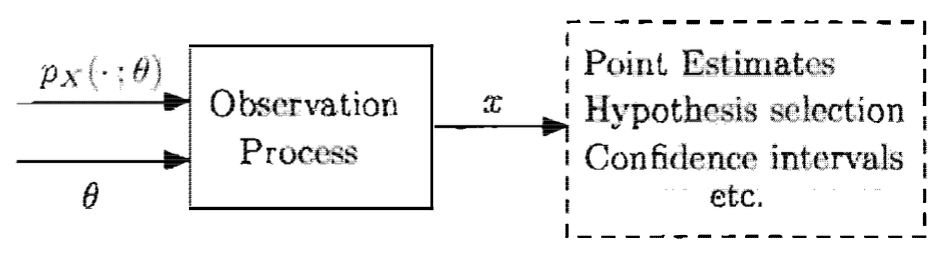
\includegraphics[width=0.5\linewidth]{figs/经典推断模型.png}
    \caption{经典推断模型}
    \label{fig:classical-inference}
\end{figure}


\subsection{经典参数估计}

\begin{definition}[估计量,估计值]
给定观测 $X=(X_1,\ldots,X_n)$,估计量指形如 $\hat\Theta_n=g(X)$ 的随机变量,估计量的取值称为估计值。注意,由于 $X$ 的分布依赖于参数 $\theta$,因而 $\hat\Theta_n$ 的分布也依赖于 $\theta$. 记 $\hat\Theta_n$ 的期望为 $\E_\theta[\hat\Theta_n]$,方差为 $\var_\theta(\hat\Theta_n)$.
\end{definition}

\begin{definition}[估计误差,偏差]
设 $\hat\Theta_n$ 是未知参数 $\theta$ 的一个估计量,定义估计误差为 $\tilde\Theta_n=\hat\Theta_n-\theta$,并定义偏差为估计误差的期望 $b_\theta(\tilde\Theta_n)=\E_\theta[\hat\Theta_n]-\theta$.
\end{definition}

\begin{definition}[无偏,渐近无偏]
若 $\E_\theta[\hat\Theta_n]=\theta$ 对 $\theta$ 所有可能的取值都成立,则称 $\hat\Theta_n$ 是无偏的;若 $\lim_{n\to\infty}\E_\theta[\hat\Theta_n]=\theta$ 对 $\theta$ 所有可能的取值都成立,则称$\hat\Theta_n$ 是渐近无偏的。
\end{definition}

\begin{definition}[相合]
若对 $\theta$ 所有可能的取值,序列 $\hat\Theta_n$ 依概率收敛到参数 $\theta$ 的真值,则称 $\hat\Theta_n$ 是 $\theta$ 的相合估计序列。
\end{definition}

\begin{property}
均方误差、偏差和 $\hat\Theta_n$ 的方差有关系:
\[
\E_\theta[\tilde\Theta_n^2]=b_\theta^2(\hat\Theta_n)+\var_\theta(\hat\Theta_n)
\]
\end{property}
\begin{remark}
这个公式很重要,等式右侧的两项体现了偏差与方差之间的权衡。
\end{remark}

\begin{definition}[极大似然估计,似然函数]
设观测向量 $X=(X_1,\ldots,X_n)$ 的联合 PMF/PDF 为 $p_X(x;\theta)$ 或 $f_X(x;\theta)$,其中 $x=(x_1,\ldots,x_n)$ 为 $X$ 的观测值。极大似然估计是使得 $p_X(x;\theta)$ 或 $f_X(x;\theta)$ 达到最大的参数值,即:
\[
\hat\theta_n=\arg\max_\theta\;p_X(x;\theta)\;\text{或}\;\arg\max_\theta\;f_X(x;\theta)
\]
称 $p_X(x;\theta)$ 或 $f_X(x;\theta)$ 为似然函数,称 $\ln p_X(x;\theta)$ 或 $\ln f_X(x;\theta)$ 为对数似然函数。
\end{definition}

\begin{remark}[极大似然估计与最大后验概率估计]
在贝叶斯最大后验概率估计中,估计的选择是使得 $p_\Theta(\theta)p_{X\vert\Theta}(x\vert\theta)$ 达到最大的 $\theta$,其中 $p_\Theta(\theta)$ 是未知参数 $\theta$ 的先验分布。因此,最大似然估计可以解释为具有均匀先验分布的最大后验概率估计。
\end{remark}

\begin{theorem}[极大似然估计的不变原理]
设 $\hat\Theta_n$ 是 $\theta$ 的极大似然估计,那么对于任意关于 $\theta$ 的一一映射函数 $h$,$h(\hat\Theta)$ 是 $\zeta=h(\theta)$ 的极大似然估计。
\end{theorem}

\begin{example}[随机变量均值的估计]
设观测值 $X_1,\ldots,X_n$ 独立同分布,均值为未知参数 $\theta$,定义样本均值为:
\[
M_n=\frac{X_1+\cdots+X_n}{n}
\]
由于 $\E_\theta[M_n]=\E_\theta[X]=\theta$,故样本均值是 $\theta$ 的无偏估计。进一步地,根据弱大数定律,$M_n$ 依概率收敛到 $\theta$,因此具有相合性。
\end{example}

\begin{example}[随机变量方差的估计]
设观测值 $X_1,\ldots,X_n$ 独立同分布,方差为未知参数 $v$,则有两个常用估计量:
\[
\bar S_n^2=\frac{1}{n}\sum\limits_{i=1}^n (X_i-M_n)^2,\qquad\hat S_n^2=\frac{1}{n-1}\sum\limits_{i=1}^n (X_i-M_n)^2
\]
可以证明 $\bar S^2$ 是有偏但渐近无偏的,$\hat S^2$ 则是无偏的。
\end{example}
\begin{proof}
注意到 $\E_{(\theta,v)}[M_n]=\theta,\,\E_{(\theta,v)}[X_i^2]=v+\theta^2,\,\E_{(\theta,v)}[M_n^2]=\frac{v}{n}+\theta^2$,于是:
\begin{align*}
\E_{(\theta,v)}[\bar S_n^2]&=\E_{(\theta,v)}\left[\frac{1}{n}\sum_{i=1}^n(X_i-M_n)^2\right]\\
&=\E_{(\theta,v)}\left[\frac{1}{n}\sum_{i=1}^nX_i^2-\frac{2M_n}{n}\sum_{i=1}^nX_i+M_n^2\right]\\
&=\E_{(\theta,v)}\left[\frac{1}{n}\sum_{i=1}^nX_i^2-2M_n^2+M_n^2\right]\\
&=v+\theta^2-\left(\frac{v}{n}+\theta^2\right)\\
&=\frac{n-1}{n}v
\end{align*}
由于 $n\to\infty$ 时 $\E_{(\theta,v)}[\bar S_n^2]\to v$,故 $\bar S_n^2$ 是渐近无偏的。又:
\[
\E_{(\theta,v)}[\hat S_n^2]=\E_{(\theta,v)}[\frac{n}{n-1}\bar S_n^2]=v
\]
故 $\hat S_n^2$ 是无偏的。
\end{proof}

\paragraph{区间估计}
在前文中,无论是贝叶斯推断中的最大后验概率估计、最小均方估计,还是经典推断中的极大似然估计,这些方法都是点估计,即给出一个数作为估计量。但有时我们还想建立一个置信区间,这就是区间估计。具体而言,我们首先固定一个\textbf{置信度} $1-\alpha$,其中 $\alpha$ 是一个很小的数。然后用一个略小的估计量 $\hat\Theta_n^-$ 和一个略大的估计量 $\hat\Theta_n^+$ 代替点估计量 $\hat\Theta_n$,使得:
\[
\Pb_\theta(\hat\Theta_n^-\leq\theta\leq\hat\Theta_n^+)\geq1-\alpha
\]
对 $\theta$ 所有可能的取值都成立。称 $[\hat\Theta_n^-,\hat\Theta_n^+]$ 为\textbf{置信区间}。

\begin{example}[正态随机变量公共均值的区间估计]
\label{ex:normal-mean-interval}
设观测量 $X_1,\ldots,X_n$ 独立同分布于 $N(\theta,v)$,其中均值 $\theta$ 未知,方差 $v$ 已知。根据例 \ref{ex:ind-normal-sum} 的结论(独立正态随机变量之和仍是正态的),可知样本均值估计量:
\[
\hat\Theta_n=\frac{X_1+\cdots+X_n}{n}\sim N\left(\theta,\frac{v}{n}\right)
\]
取 $\alpha=0.05$,即置信度 $0.95$,查正态分布表可得 $\Phi(1.96)=0.975=1-\alpha/2$,于是:
\[
\Pb_\theta\left(\left|\frac{\hat\Theta_n-\theta}{\sqrt{v/n}}\right|\leq1.96\right)=\Pb_\theta\left(\hat\Theta_n-1.96\sqrt{\frac{v}{n}}\leq\theta\leq \hat\Theta_n+1.96\sqrt{\frac{v}{n}}\right)=0.95
\]
这说明:
\[
\left[\hat\Theta_n-1.96\sqrt{\frac{v}{n}},\;\hat\Theta_n+1.96\sqrt{\frac{v}{n}}\right]
\]
是 $95\%$ 置信区间。
\end{example}

\begin{example}[基于方差近似估计量的区间估计]
设观测量 $X_1,\ldots,X_n$ 独立同分布于 $N(\theta,v)$,其中均值 $\theta$ 和方差 $v$ 都是未知的。考虑用方差的无偏估计量:
\[
\hat S_n^2=\frac{1}{n-1}\sum_{i=1}^n(X_i-\hat\Theta_n)^2
\]
代替方差,则根据例 \ref{ex:normal-mean-interval} 和中心极限定理,可构造一个近似的 $1-\alpha$ 置信区间:
\[
\left[\hat\Theta_n-z\frac{\hat S_n}{\sqrt{n}},\;\hat\Theta_n+z\frac{\hat S_n}{\sqrt{n}}\right]
\]
其中 $z$ 满足 $\Phi(z)=1-\alpha/2$. 例如,近似 $95\%$ 置信区间为:
\[
\left[\hat\Theta_n-1.96\frac{\hat S_n}{\sqrt{n}},\;\hat\Theta_n+1.96\frac{\hat S_n}{\sqrt{n}}\right]
\]
事实上,当用 $\hat S_n^2$ 代替方差后,随机变量:
\[
T_n=\frac{\sqrt{n}(\hat\Theta_n-\theta)}{\hat S_n}
\]
服从自由度为 $n-1$ 的 $t$ 分布(详见附录 \ref{sec:normal-derive})。因此,设 $t$ 分布的分布函数为 $\Psi_{n-1}(z)$,则更精确的置信区间中,$z$ 应满足 $\Psi_{n-1}(z)=1-\alpha/2$. 
\end{example}

\begin{definition}[充分统计量]
给定观测 $X=(X_1,\ldots,X_n)$,设随机变量 $T=q(X)$ 为 关于 $X$ 的标量或向量函数,若 $X$ 在给定 $T$ 下的条件分布不依赖于 $\theta$,即:
\[
\Pb_\theta(X\in D\vert T=t),\quad\forall\,t
\]
对所有 $\theta$ 都是一样的,则称 $T$ 为 $\theta$ 的充分统计量。
\end{definition}

\begin{theorem}[因子分解定理]
\label{thm:factorization}
$T=q(X)$ 是 $\theta$ 的充分统计量当且仅当似然函数 $p_X(x;\theta)$ 或 $f_X(x;\theta)$ 可以写成 $r(q(x),\theta)s(x)$ 的形式,其中 $r,s$ 是两个函数。
\end{theorem}
\begin{proof}
假设 $X$ 是离散随机变量,连续情形类似。首先证明充分性。假设 $p_X(x;\theta)=r(q(x),\theta)s(x)$,取定 $T=t$,则对所有 $q(x)\neq t$ 的 $x$,容易知道:
\[
\Pb_\theta(X=x\vert T=t)=\frac{\Pb_\Theta(X=x)\Pb_\theta(T=t\vert X=x)}{\Pb_\theta(T=t)}=0
\]
而对于满足 $q(x)=t$ 的 $x$,有:
\begin{align*}
\Pb_\theta(X=x\vert T=t)&=\frac{\Pb_\theta(X=x,T=t)}{\Pb_\theta(T=t)}=\frac{\Pb_\theta(X=x)}{\Pb_\theta(T=t)}=\frac{\Pb_\theta(X=x)}{\sum_z\Pb_\theta(X=z,T=t)}\\
&=\frac{\Pb_\theta(X=x)}{\sum_{\{z\mid q(z)=t\}}\Pb_\theta(X=z)}=\frac{r(q(x),\theta)s(x)}{\sum_{\{z\mid q(z)=t\}}r(q(z),\theta)s(z)}\\
&=\frac{r(t,\theta)s(x)}{r(t,\theta)\sum_{\{z\mid q(z)=t\}}s(z)}=\frac{s(x)}{\sum_{\{z\mid q(z)=t\}}s(z)}
\end{align*}
可见对所有 $x$,$\Pb_\theta(X=x\vert T=t)$ 都不依赖于 $\theta$,故 $T$ 是充分统计量。

然后证明必要性。设 $T=q(X)$ 是 $\theta$ 的充分统计量,则对任意 $x$,有:
\[
p_X(x;\theta)=\sum_t\Pb_\theta(X=x\vert T=t)\Pb_\theta(T=t)=\Pb_\theta(X=x\vert T=q(x))\Pb_\theta(T=q(x))
\]
右式两部分中,前者与 $\theta$ 无关,故可写作 $s(x)$ 的形式,而后者为 $r(q(x),\theta)$ 的形式。
\end{proof}

\begin{theorem}
若 $q(X)$ 是 $\theta$ 的充分统计量,则对 $\theta$ 的任何函数 $h$,$q(X)$ 都是 $\zeta=h(\theta)$ 的充分统计量。
\end{theorem}
\begin{proof}
对 $\zeta=h(\theta)$ 有:
\[
\Pb_{\zeta}(X\in D\vert T=t)=\Pb_{\theta}(X\in D\vert T=t)
\]
所以 $\Pb_{\zeta}(X\in D\vert T=t)$ 对所有 $\zeta$ 都是一样的。
\end{proof}

\begin{theorem}
若 $q(X)$ 是 $\theta$ 的充分统计量,则 $\theta$ 的极大似然估计可以写作 $\hat\Theta_n=\phi(q(X))$.
\end{theorem}
\begin{proof}
根据因子分解定理 \ref{thm:factorization},$p_X(x;\theta)=r(q(x),\theta)s(x)$,故极大似然估计为:
\[
\hat\theta_n=\arg\max_\theta\;p_X(x;\theta)=\begin{dcases}
    \arg\max_\theta\;r(q(x),\theta),&\text{$s(x)>0$}\\
    \arg\min_\theta\;r(q(x),\theta),&\text{$s(x)<0$}
\end{dcases}
\]
即 $\hat\theta_n$ 只通过 $\phi(q(x))$ 依赖于 $x$,故 $\hat\Theta_n=\phi(q(X))$.
\end{proof}
\begin{remark}
该定理说明充分统计量抓住了由 $X$ 提供的关于 $\theta$ 的所有核心信息。
\end{remark}

\begin{example}[伯努利分布]
设 $X_1,\ldots,X_n$ 独立同分布于参数为 $\theta$ 的伯努利分布,则:
\[
q(X)=\sum_{i=1}^nX_i
\]
是 $\theta$ 的充分统计量。这是因为似然函数为:
\[
p_X(x;\theta)=\theta^{\sum_{i=1}^n x_i}(1-\theta)^{n-\sum_{i=1}^nx_i}=\theta^{q(x)}(1-\theta)^{n-q(x)}
\]
可以分解为 $r(q(x),\theta)=\theta^{q(x)}(1-\theta)^{n-q(x)}$ 与常函数 $s(x)=1$ 的乘积。
\end{example}

\begin{example}[泊松分布]
设 $X_1,\ldots,X_n$ 独立同分布于参数为 $\theta$ 的泊松分布,则:
\[
q(X)=\sum_{i=1}^nX_i
\]
是 $\theta$ 的充分统计量。这是因为似然函数为:
\[
p_X(x;\theta)=\prod_{i=1}^np_{X_i}(x_i;\theta)=e^{-\theta}\prod_{i=1}^n\frac{\theta^{x_i}}{x_i!}=e^{-\theta}\frac{\theta^{q(x)}}{\prod_{i=1}^nx_i!}
\]
可以分解为 $r(q(x),\theta)=e^{-\theta}\theta^{q(x)}$ 与 $s(x)=1/\prod_{i=1}^nx_i!$ 的乘积。
\end{example}

\begin{example}[正态分布]
设 $X_1,\ldots,X_n$ 独立同分布于 $N(\mu,\sigma^2)$,则:
\begin{itemize}
    \item 若 $\sigma^2$ 已知,则 $q(X)=\sum_{i=1}^nX_i$ 是 $\mu$ 的充分统计量。
    \item 若 $\mu$ 已知,则 $q(X)=\sum_{i=1}^n(X_i-\mu)^2$ 是 $\sigma^2$ 的充分统计量。
    \item 若 $\mu,\sigma^2$ 都未知,则 $q(X)=(\sum_{i=1}^nX_i,\sum_{i=1}^nX_i^2)$ 是 $(\mu,\sigma^2)$ 的充分统计量。
\end{itemize}
\end{example}

\begin{theorem}[Rao-Blackwell]
给定观测 $X=(X_1,\ldots,X_n)$,设 $T=q(X)$ 是参数 $\theta$ 的充分估计量,$g(X)$ 是 $\theta$ 的一个估计量。则:
\begin{enumerate}
    \item $\E_\theta[g(X)\vert T]$ 对所有 $\theta$ 都一样,因而可以去掉下标 $\theta$,将:
    \[
    \hat g(X)=\E[g(X)\vert T]
    \]
    视作 $\theta$ 的一个新估计量,它只通过 $T$ 依赖于 $X$.
    \item 新估计量 $\hat g(X)$ 与原估计量 $g(X)$ 偏差相等。
    \item 对满足 $\var_\theta(g(X))<\infty$ 的 $\theta$,有均方误差:
    \[
    \E_\theta[(\hat g(X)-\theta)^2]\leq\E_\theta[(g(X)-\theta)^2]
    \]
    进一步地,给定 $\theta$,此不等式是严格的当且仅当:
    \[
    \E_\theta[\var(g(X)\vert T)]>0
    \]
\end{enumerate}
\end{theorem}
\begin{proof}
我们逐条证明:
\begin{enumerate}
    \item 由于 $T$ 是充分估计量,所以条件分布 $\Pb_\theta(X=x\vert T=t)$ 不依赖于 $\theta$,自然 $\E_\theta[g(X)\vert T]$ 不依赖于 $\theta$.
    \item 根据全期望公式,有:
    \[
    \E_\theta[\hat g(X)]=\E[\E[g(X)\vert T]]=\E_\theta[g(X)]
    \]
    因而偏差相等:
    \[
    \E_\theta[\hat g(x)]-\theta=\E_\theta[g(x)]-\theta
    \]
    \item 对于固定的 $\theta$,记 $\hat g(X)$ 和 $g(X)$ 的偏差为 $b_\theta$. 根据全方差公式,有:
    \begin{align*}
    \E_\theta[(g(X)-\theta)^2]&=\var_\theta(g(X))+b_\theta^2\\
    &=\E_\theta[\var(g(X)\vert T)]+\var_\theta(\E[g(X)\vert T])+b_\theta^2\\
    &=\E_\theta[\var(g(X)\vert T)]+\var_\theta(\hat g(X))+b_\theta^2\\
    &=\E_\theta[\var(g(X)\vert T)]+\E_\theta[(\hat g(X)-\theta)^2]\\
    &\geq\E_\theta[(\hat g(X)-\theta)^2]
    \end{align*}
    且不等式是严格的当且仅当 $\E_\theta[\var(g(X)\vert T)]>0$.
\end{enumerate}
\end{proof}
\begin{remark}
Rao-Blackwell 定理说明,一个一般的估计量可以改进为一个只依赖于充分统计量的估计量,新的估计量偏差与原估计量相同,但均方误差更小。
\end{remark}

\begin{example}
设 $X_1,\ldots,X_n$ 是 $[0,\theta]$ 上独立同分布的均匀随机变量。
\begin{enumerate}[label=(\alph*)]
    \item 证明 $T=\max_{i=1,\ldots,n}X_i$ 是充分统计量。
    \item 证明 $g(X)=(2/n)\sum_{i=1}^nX_i$ 是无偏估计。
    \item 找出估计量 $\hat g(X)=\E[g(X)\vert T]$ 的形式,计算并比较 $\E_\theta[(\hat g(X)-\theta)^2]$ 和 $\E_\theta[(g(X)-\theta)^2]$.
\end{enumerate}
\end{example}
\begin{proof}
\,
\begin{enumerate}[label=(\alph*)]
    \item 由于似然函数为:
    \[
    f_X(x_1,\ldots,x_n;\theta)=\begin{cases}
    1/\theta^n,&0\leq \max_{i=1,\ldots,n}x_i\leq\theta\\
    0,&\text{otherwise}
    \end{cases}
    \]
    只通过 $\max_{i=1,\ldots,n}x_i$ 依赖于 $x$,根据因子分解定理可知其为充分统计量。
    \item 由于:
    \[
    \E_\theta[g(X)]=\frac{2}{n}\sum_{i=1}^n\E_\theta[X_i]=\frac{2}{n}\sum_{i=1}^n\frac{\theta}{2}=\theta
    \]
    故 $g(X)$ 是无偏估计。
    \item 固定 $T=t$,则 $X_1,\ldots,X_n$ 中有一个等于 $t$,其余观测服从 $[0,t]$ 上的均匀分布,因此:
    \[
    \E[g(X)\vert T=t]=\frac{2}{n}\E_\theta\left[\sum_{i=1}^nX_i\vert T=t\right]=\frac{2}{n}\left(t+(n-1)\frac{t}{2}\right)=\frac{n+1}{n}t
    \]
    所以:
    \[
    \hat g(X)=\E[g(X)\vert T]=\frac{n+1}{n}T
    \]
    下面计算均方误差。首先计算一阶矩:
    \[
    \E_\theta[\hat g(X)]=\E_\theta[\E[g(X)\vert T]]=\E_\theta[g(X)]=\theta
    \]
    可以看出 $\hat g(X)$ 也是无偏估计,这符合 Rao-Blackwell 定理的第二点。为了计算二阶矩,需要首先确定 $T$ 的分布:
    \[
    F_T(t;\theta)=\Pb_\theta(T\leq t)=\left(\frac{t}{\theta}\right)^n\implies f_T(t;\theta)=\frac{nt^{n-1}}{\theta^n},\quad t\in[0,\theta]
    \]
    于是:
    \[
    \E_\theta[(\hat g(X))^2]=\left(\frac{n+1}{n}\right)^2\E_\theta\left[T^2\right]=\left(\frac{n+1}{n}\right)^2\int_0^\theta t^2\frac{nt^{n-1}}{\theta^n}\mathrm dt=\frac{(n+1)^2}{n(n+2)}\theta^2
    \]
    由于 $\hat g(X)$ 是无偏估计,所以均方误差就是方差:
    \[
    \E_\theta[(\hat g(X)-\theta)^2]=\E_\theta[(\hat g(X))^2]-\theta^2=\frac{(n+1)^2}{n(n+2)}\theta^2-\theta^2=\frac{\theta^2}{n(n+2)}
    \]
    同理,$g(X)$ 均方误差也是其方差,且:
    \[
    \E_\theta[(g(X)-\theta)^2]=\var_\theta(g(X))=\frac{4}{n^2}\sum_{i=1}^n\var_\theta(X_i)=\frac{4}{n^2}\sum_{i=1}^n\frac{\theta^2}{12}=\frac{\theta^2}{3n}
    \]
    由于 $n(n+2)\geq 3n,\;\forall n>0$,所以:
    \[
    \E_\theta[(\hat g(X)-\theta)^2]\leq\E_\theta[(g(X)-\theta)^2]
    \]
    即我们得到了一个方差更小的无偏估计。这符合 Rao-Blackwell 定理的第三点。
\end{enumerate}
\end{proof}


\subsection{线性回归}

线性回归为两个或多个变量建立线性模型,可以由\textbf{最小二乘法}完成而不需要任何概率上的解释,但也可以在各种概率框架下进行解释。

\paragraph{一元线性回归}
设有 $n$ 个数据对 $(x_i,y_i),\,i=1,\ldots,n$,建立线性模型:
\[
y\approx\theta_0+\theta_1 x
\]
其中 $\theta_0,\theta_1$ 是未知的待估计参数。特别地,给定参数的估计 $\hat\theta_0,\hat\theta_1$,则模型对 $x_i$ 的估计为:
\[
\hat y_i=\hat\theta_0+\hat\theta_1 x_i
\]
其与真实值 $y_i$ 之间的差异称作残差:
\[
\tilde y_i=y_i-\hat y_i
\]
线性回归的优化目标是最小化残差的平方和:;
\[
\min_{\theta_0,\theta_1}\quad \sum_{i=1}^n(y_i-\hat y_i)^2=\sum_{i=1}^n(y_i-\theta_0-\theta_1 x_i)^2
\]
这是关于 $\theta_0,\theta_1$ 的二次函数,容易求得最优估计为:
\[
\hat\theta_1=\frac{\sum\limits_{i=1}^n(x_i-\bar x)(y_i-\bar y)}{\sum\limits_{i=1}^n(x_i-\bar x)^2},\quad\hat\theta_0=\bar y-\hat\theta_1\bar x
\]
其中,
\[
\bar x=\frac{1}{n}\sum_{i=1}^n x_i,\quad \bar y=\frac{1}{n}\sum_{i=1}^ny_i
\]

\paragraph{概率框架解释·极大似然}
对于每个 $x_i$,将 $y_i$ 视作随机变量 $Y_i$ 的一个取值。设 $Y_i$ 的模型为:
\[
Y_i=\theta_0+\theta_1 x_i+W_i,\;i=1,\ldots,n
\]
其中 $W_i$ 是均值为零、方差为 $\sigma^2$ 的正态独立同分布随机变量,因而 $Y_i$ 也是独立的正态随机变量且 $Y_i\sim N(\theta_0+\theta_1 x_i,\sigma^2)$. 于是似然函数为:
\[
f_Y(y;\theta)=\prod_{i=1}^n\frac{1}{\sqrt{2\pi}\sigma}\exp\left\{-\frac{(y_i-\theta_0-\theta_1 x_i)^2}{2\sigma^2}\right\}
\]
当似然函数最大时,指数部分达到最大,即残差平方和最小。因此最小二乘法可以视为 $Y$ 的期望具有线性结构的正态模型中参数 $\theta_0,\theta_1$ 的极大似然估计。

\paragraph{概率框架解释·近似贝叶斯线性最小均方估计}
将 $x_i,y_i$ 都视作随机变量 $X_i,Y_i$ 的取值,设不同 $(X_i,Y_i)$ 之间是独立同分布的,但是它们的二维联合分布未知。考虑服从同一分布的另一随机变量对 $(X_0,Y_0)$,假设观测到 $X_0$ 并希望用线性估计量 $\hat Y_0=\theta_0+\theta_1 X_0$ 来估计 $Y_0$. 根据定理 \ref{thm:linear-lms-estimate},$Y_0$ 的线性最小均方估计量为:
\[
\hat Y_0=\E Y_0+\frac{\cov(Y_0,X_0)}{\var(X_0)}(X_0-\E X_0)
\]
也即:
\[
\theta_1=\frac{\cov(Y_0,X_0)}{\var(X_0)},\quad\theta_0=\E Y_0-\theta_1\E X_0
\]
由于我们不知道 $(X_0,Y_0)$ 的分布,因此作估计:
\[
    \E X_0\approx\bar x,\quad
    \E Y_0\approx\bar y,\quad
    \cov(Y_0,X_0)\approx\frac{1}{n}\sum_{i=1}^n(x_i-\bar x)(y_i-\bar y),\quad
    \var(X_0)\approx\frac{1}{n}\sum_{i=1}^n(x_i-\bar x)^2
\]
代入即可得到最小二乘公式。

\paragraph{概率框架解释·近似贝叶斯最小均方估计}

仍然假设 $(X_i,Y_i)$ 独立同分布,并附加新的假设——数据满足模型:
\[
Y_i=\theta_0+\theta_1X_i+W_i
\]
其中 $W_i$ 是独立同分布的零均值噪声项且与 $X_i$ 独立。根据定理 \ref{thm:lms-overall} 可知,$Y_0$ 的最小均方估计量为:
\[
\E[Y_0\vert X_0]=\E[\theta_0+\theta_1X_0+W_0\vert X_0]=\theta_0+\theta_1X_0
\]
换句话说,$\theta_0+\theta_1X_0$ 是所有关于 $X_0$ 的函数 $g(X_0)$ 中使得均方误差最小的,于是:
\[
\theta_0,\theta_1=\argmin_{\theta_0',\theta_1'}\;\E[(Y_0-\theta_0'-\theta_1'X_0)^2]
\]
注意到,根据弱大数定律,当 $n\to\infty$ 时,上式是:
\[
\frac{1}{n}\sum_{i=1}^n(Y_i-\theta_0'-\theta_1'X_i)^2
\]
的极限,而该式正是最小二乘法的优化目标。

\paragraph{贝叶斯线性回归}
将 $x_1,\ldots,x_n$ 视为给定的数,将 $(y_1,\ldots,y_n)$ 视为随机向量 $Y=(Y_1,\ldots,Y_n)$ 的观测值,且假设有线性关系:
\[
Y_i=\Theta_0+\Theta_1x_i+W_i
\]
其中 $\Theta=(\Theta_0,\Theta_1)$ 是待估计的参数(视为随机变量)。假设 $\Theta_0,\Theta_1,W_1,\ldots,W_n$ 是相互独立的正态随机变量。$W_1,\ldots,W_n$ 均值为零,方差已知为 $\sigma^2$. $\Theta_0,\Theta_1$ 的均值为零,方差分别为 $\sigma_0^2,\sigma_1^2$. 则根据贝叶斯公式,后验概率密度函数为:
\begin{align*}
f_{\Theta\vert Y}(\theta_0,\theta_1\vert y_1,\ldots,y_n)&\propto f_\Theta(\theta_0,\theta_1)f_{Y\vert\Theta}(y_1,\ldots,y_n\vert \theta_0,\theta_1)\\
&\propto\exp\left(-\frac{\theta_0^2}{2\sigma_0^2}\right)\cdot\exp\left(-\frac{\theta_1^2}{2\sigma_1^2}\right)\prod_{i=1}^n\cdot\exp\left(-\frac{y_i^2}{2\sigma^2}\right)\\
&\propto\exp\left(-\left(\frac{\theta_0^2}{2\sigma_0^2}+\frac{\theta_1^2}{2\sigma_1^2}+\sum_{i=1}^n\frac{y_i^2}{2\sigma^2}\right)\right)
\end{align*}
因此,最大后验概率估计就是:
\[
\hat\theta_0,\hat\theta_1=\argmin_{\theta_0,\theta_1}\;\left(\frac{\theta_0^2}{2\sigma_0^2}+\frac{\theta_1^2}{2\sigma_1^2}+\sum_{i=1}^n\frac{y_i^2}{2\sigma^2}\right)
\]
求导并令导数为零,可解得:
\[
    \hat\theta_1=\frac{\sigma_1^2}{\sigma^2+\sigma_1^2\sum_{i=1}^n(x_i-\bar x)^2}\cdot\sum_{i=1}^n(x_i-\bar x)(y_i-\bar y),\quad\hat\theta_0=\frac{n\sigma_0^2}{\sigma^2+n\sigma_0^2}(\bar y-\hat\theta_1\bar x)
\]

\paragraph{多元线性回归}
一元线性回归可以直接扩展到多元情形。例如,设数据由三元组 $(x_i,y_i,z_i)$ 组成,建立线性模型:
\[
y\approx\theta_0+\theta_1x+\theta_2z
\]
则多元线性回归最小化残差的平方和:
\[
\min_{\theta_0,\theta_1,\theta_2}\quad\sum_{i=1}^n(y_i-\theta_0-\theta_1x_i-\theta_2z_i)^2
\]

特别地,$z$ 可以是 $x$ 的函数,例如 $z=x^2$. 尽管二次函数不是线性的,但是未知参数 $\theta_j$ 与随机变量 $Y_i$ 是线性关系,所以这仍然属于线性回归的范畴。一般地,考虑如下形式的模型:
\[
y\approx\theta_0+\sum_{j=1}^m\theta_jh_j(x)
\]
则回归问题的优化目标为:
\[
\min_{\theta_0,\ldots,\theta_m}\quad\sum_{i=1}^n\left(y_i-\theta_0-\sum_{j=1}^m\theta_jh_j(x_i)\right)^2
\]
这样的最小化问题都有现存的公式。


\subsection{简单假设检验}

在经典统计推断中,我们不再有先验概率的假设,因此假设检验问题可以看作是 $\theta$ 只有两个取值的推断问题。我们一般用 $H_0$ 表示\textbf{原假设},$H_1$ 表示\textbf{备择假设}。

设观测随机变量 $X=(X_1,\ldots,X_n)$,记 $\Pb(X\in A;H_j)$ 表示假设 $H_j$ 成立时 $X$ 属于 $A$ 的概率。类似地,记 $p_X(x;H_j)$ 或 $f_X(x;H_j)$ 表示假设 $H_j$ 成立时的 PMF 或 PDF. 我们希望找到一个决策准则将观测值 $x$ 映射到其中一个假设上去。任何一个决策准则都将样本空间划分为了两个区域——拒绝域与接受域。当观测数据落入拒绝域时,称假设 $H_0$ 被拒绝,反之则被接受。

一个决策准则有两种错误。设该决策准则决定的拒绝域为 $R$,第一类错误指拒绝了 $H_0$ 但它实际上是正确的,此类错误发生概率为 $\alpha(R)=\Pb(x\in R;H_0)$;第二类错误指接受了 $H_0$ 但它实际上是错误的,此类错误发生概率为 $\beta(R)=\Pb(x\not\in R;H_1)$.

\begin{definition}[似然比]
定义似然比为:
\[
L(x)=\frac{p_X(x;H_1)}{p_X(x;H_0)}\quad\text{或}\quad L(x)=\frac{f_X(x;H_1)}{f_X(x;H_0)}
\]
\end{definition}

基于似然比的概念,我们可以得到这样的决策准则:选择一个临界值 $\xi\in(0,\infty)$,当观测值 $x$ 满足 $L(x)>\xi$ 时,拒绝原假设 $H_0$. 特别地,当 $\xi=1$ 时,我们总是选择似然最大的假设,此时正好对应极大似然准则。

\paragraph{似然比检验}
首先确定错误拒绝的概率 $\alpha$,然后选择一个常数 $\xi$,使得错误拒绝的概率为 $\alpha$:
\[
\Pb(L(x)>\xi;H_0)=\alpha
\]
那么拒绝域就是 $R=\{x\mid L(x)>\xi\}$. 当观测值落入拒绝域中时,即 $L(x)>\xi$ 时,我们拒绝 $H_0$.

\begin{lemma}[Neyman-Pearson 引理]
考虑似然比检验中一个确定的 $\xi$,从而有犯错概率:
\[
\Pb(L(X)>\xi;H_0)=\alpha,\quad\Pb(L(X)\leq\xi;H_1)=\beta
\]
假设还有其他检验,拒绝域为 $R$,使得错误拒绝的概率一样或更小:
\[
\Pb(X\in R;H_0)\leq\alpha
\]
那么这个检验错误接受的概率一样或更大:
\[
\Pb(X\not\in R;H_1)\geq\beta
\]
当 $\Pb(X\in R;H_0)<\alpha$ 严格成立时,$\Pb(X\not\in R;H_1)>\beta$ 严格成立。
\end{lemma}


\subsection{显著性检验}

在实际情况中,假设检验问题并不总是只有两个特定的选择,因而简单假设检验的方法可能不再使用。本节介绍更一般的问题和解决方法。

假设观测 $X=(X_1,\ldots,X_n)$ 服从由参数 $\theta$ 决定的 PMF/PDF,其中 $\theta$ 在给定集合 $\mathcal M$ 中取值。我们称“断言 $\theta$ 的真值为 $\theta_0\in\mathcal M$” 为原假设,记作 $H_0$,而相应的 $\theta\neq\theta_0$ 为备择假设,记作 $H_1$.

\paragraph{显著性检验}
基于观测 $X_1,\ldots,X_n$,对假设 $H_0:\theta=\theta_0$ 做统计检验:
\begin{enumerate}
    \item 选择统计量 $S=h(X_1,\ldots,X_n)$,其中 $h:\mathbb R^n\to\mathbb R$.
    \item 确定拒绝域形状:拒绝域 $R$ 为 $S$ 的取值的子集,当 $S$ 落入 $R$ 时就拒绝 $H_0$;这个过程通常涉及一个常数 $\xi$,称作临界值;
    \item 选择显著水平 $\alpha$;
    \item 选择临界值 $\xi$ 使得错误拒绝的概率等于或约等于 $\alpha$;此时拒绝域 $R$ 就完全确定了;
    \item 得到 $X_1,\ldots,X_n$ 的观测值 $x_1,\ldots,x_n$,计算统计值 $s=h(x_1,\ldots,x_n)$,若 $s$ 落入 $R$ 则拒绝 $H_0$.
\end{enumerate}

\begin{com}
很多时候,统计学家并不选择显著水平 $\alpha$ 和临界值 $\xi$,而是计算统计值 $s$ 后,直接汇报 $p$-值:
\[
    p\text{-值}=\min\{\alpha\mid H_0\,\text{在显著水平 $\alpha$ 下被拒绝}\}
\]
\end{com}

